%=====================================================================
%  06-ENTROPI.TEX — ENTROPI (TEORI INFORMASI & KUANTUM)
%=====================================================================
\section{ENTROPY}

%---------------------------------------------------------------------
%  Entropy 1/3 — empat konsep dasar entropi klasik, dua kolom.
%---------------------------------------------------------------------
\begin{frame}
    \frametitle{Entropy 1/3}
    \vspace*{-0.5cm}
    \begin{columns}[T]
        \small
        \begin{column}{0.5\textwidth}
            \begin{itemize}\tiny\justifying
                \item Entropi \cite{djordjevic2019physical}
                    \begin{itemize}
                        \item[$\Rightarrow$] Ukuran ketidakpastian/kekacauan suatu
                            sistem atau distribusi probabilitas; dalam teori
                            informasi mengukur banyaknya informasi yang
                            terkandung dalam suatu variabel acak.
                        \item[$\Rightarrow$] Semakin tinggi entropi suatu sistem,
                            semakin tinggi ketidakpastiannya.
                    \end{itemize}
                \item Conditional Entropy
                    \begin{itemize}
                        \item[$\Rightarrow$] Ketidakpastian yang tersisa pada input
                            saluran setelah output saluran diterima.
                        \item[$\Rightarrow$] Diukur melalui
                            $H(Y|X)=-\sum_{x\in X}p(x)\sum_{y\in Y}p(y|x)\log p(y|x)$
                            dengan $p(x,y)$ \textit{joint distribution} input
                            dan output saluran.
                    \end{itemize}
            \end{itemize}
        \end{column}

        \begin{column}{0.5\textwidth}
            \begin{itemize}\tiny\justifying
                \item Relative Entropy \cite{wolfowitz2012coding}
                    \begin{itemize}
                        \item[$\Rightarrow$] Jarak Kullback--Leibler (KL) antara
                            dua distribusi: mengukur ketidakefisienan dengan
                            mengasumsikan $q(x)$ padahal sebenarnya $p(x)$:
                            $D(p\,\|\,q)=\sum_x p(x)\log\!\left(p(x)/q(x)\right)$.
                    \end{itemize}
                \item Mutual Information \cite{djordjevic2019physical}
                    \begin{itemize}
                        \item[$\Rightarrow$] Banyaknya informasi yang dikandung
                            satu variabel acak tentang variabel acak lain;
                            informasi input yang diketahui setelah melihat
                            output saluran.
                        \item[$\Rightarrow$] $I(X;Y)=H(X)-H(X|Y)$ dengan $H(X)$
                            entropi output dan $H(X|Y)$ conditional entropy.
                    \end{itemize}
            \end{itemize}
        \end{column}
    \end{columns}
\end{frame}

%---------------------------------------------------------------------
%  Entropy 2/3 — diagram entropi, von Neumann, negative conditional.
%---------------------------------------------------------------------
\begin{frame}
    \frametitle{Entropy 2/3}
    \vspace*{-0.5cm}
    \begin{columns}[T]
        \small
        \begin{column}{0.5\textwidth}
            \begin{figure}
                \centering
                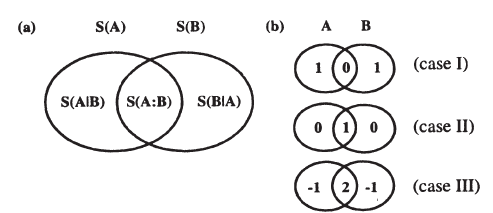
\includegraphics[width=0.96\textwidth]{gambar/DIAGRAM/diagram2.png}
                \captionsetup{font=tiny, justification=justified, width=0.96\textwidth}
                \captionof{figure}{(a) Diagram entropi umum untuk sistem komposit
                kuantum AB. (b) Diagram entropi tiga kasus sistem 2-qubit:
                (I) independen, (II) terkorelasi klasik, (III) kuantum
                \textit{entanglement}.}
                \label{fig:diagram-entropi}
            \end{figure}
            \begin{itemize}\tiny\justifying
                \vspace{-0.6cm}
                \item Entropi von Neumann, Persamaan~\ref{eq:entropi-vonneumann},
                    diperkenalkan dalam mekanika kuantum dan terkait dengan
                    entropi Boltzmann--Gibbs--Shannon,
                    Persamaan~\ref{eq:entropi-bgs}, pada situasi klasik tertentu.
                    \begin{equation}
                        S(\rho)=-\Tr(\rho\log\rho)
                        \label{eq:entropi-vonneumann}
                    \end{equation}
                    \begin{equation}
                        H(p)=-\sum_i P_i\log P_i
                        \label{eq:entropi-bgs}
                    \end{equation}
            \end{itemize}
        \end{column}

        \begin{column}{0.5\textwidth}
            \begin{itemize}\tiny\justifying
                \item Matriks densitas subsistem AB \\
                    Melacak (mengabaikan) derajat kebebasan C dari sistem
                    ABC memberikan matriks densitas marginal subsistem AB
                    \begin{equation}
                        \rho_{AB}=\Tr_C[\rho_{ABC}]
                        =\tfrac{1}{2}\left(\ketbra{00}{00}+\ketbra{11}{11}\right),
                        \label{eq:matriks-densitas-AB}
                    \end{equation}
                    yang sesuai dengan sistem klasik yang berkorelasi.
                \item Negative Entropy \\
                    Memasukkan Persamaan~\ref{eq:matriks-densitas-AB} ke dalam
                    Persamaan~\ref{eq:entropi-vonneumann} menghasilkan
                    $S(A|B)=-1$. Entropi kondisional dituliskan sebagai
                    \begin{equation}
                        S(A|B)\equiv S(AB)-S(B).
                    \end{equation}
                \item Fungsi Negative Conditional Entropy \\
                    Pada sistem kuantum komposit, konsep entropi kondisional
                    negatif terbukti sangat berguna menjelaskan sistem kuantum
                    multibagian, serta memberi pemahaman baru tentang pembentukan
                    korelasi klasik dari \textit{quantum entanglement}
                    \cite{cerf1997negative}.
            \end{itemize}
        \end{column}
    \end{columns}
\end{frame}

%---------------------------------------------------------------------
%  Entropy 3/3 — contoh perhitungan lengkap entropi negatif.
%  PERBAIKAN dari versi lama (kesalahan notasi/tulis):
%    * amplitudo Bell state 1/2 -> 1/sqrt(2) (agar ter-normalisasi);
%    * \ket{...}){AB} -> subskrip benar _{AB};
%    * "tr B (\rho{AB})" -> \Tr_B(\rho_{AB});
%    * faktor 1/2 pada proyektor konsisten dengan (1/sqrt(2))^2 = 1/2;
%    * I_A (1/2) \otimes I_B (1/2) -> (1/2 I_A) \otimes (1/2 I_B).
%---------------------------------------------------------------------
\begin{frame}
    \frametitle{Entropy 3/3 --- Contoh: Keadaan Bell $ \ket{\psi_{AB}} $}
    \vspace*{-0.5cm}
    \begin{columns}[T]
        \tiny
        \begin{column}{0.5\textwidth}
            % Keadaan Bell ter-normalisasi: amplitudo 1/sqrt(2)
            \begin{align*}
                \ket{\psi_{AB}} &= \frac{1}{\sqrt{2}}\left(\ket{00}+\ket{11}\right)_{AB}\\[2pt]
                \rho_{AB} &= \ketbra{\psi_{AB}}{\psi_{AB}}\\
                &= \frac{1}{2}\left(\ket{00}+\ket{11}\right)_{AB}
                   \left(\bra{00}+\bra{11}\right)_{AB}\\
                &= \frac{1}{2}\left(\ketbra{00}{00}+\ketbra{00}{11}
                   +\ketbra{11}{00}+\ketbra{11}{11}\right)
            \end{align*}
            % Reduced matrix: lacak (trace) subsistem B
            \begin{align*}
                \hat{\rho}_A &= \Tr_B(\rho_{AB})\\
                &= \frac{1}{2}\left(
                   |0\rangle\langle 0|_A\,\Tr\!\left(\ketbra{0}{0}\right)
                 + |0\rangle\langle 1|_A\,\Tr\!\left(\ketbra{0}{1}\right)\right.\\
                &\quad\; +\left.
                   |1\rangle\langle 0|_A\,\Tr\!\left(\ketbra{1}{0}\right)
                 + |1\rangle\langle 1|_A\,\Tr\!\left(\ketbra{1}{1}\right)\right)\\
                &= \frac{1}{2}\left(|0\rangle\langle 0|_A
                   +|1\rangle\langle 1|_A\right)\\
                &\equiv \frac{1}{2}I_A
            \end{align*}
        \end{column}

        \begin{column}{0.5\textwidth}
            \begin{align*}
                \hat{\rho}_B &= \Tr_A(\rho_{AB})
                    \equiv \tfrac{1}{2}I_B\\
                \hat{\rho}_A\otimes\hat{\rho}_B
                    &= \left(\tfrac{1}{2}I_A\right)\otimes\left(\tfrac{1}{2}I_B\right)
                     \equiv \tfrac{1}{4}I_{AB}\\
                S(\hat{\rho}_A) &= S(\hat{\rho}_B)
                    = -2\times\tfrac{1}{2}\log\tfrac{1}{2} \equiv 1\\
                S(\rho_{AB}) &= 0 \quad\text{(keadaan murni)}\\
                S(\rho_A|\rho_B) &= S(\rho_{AB})-S(\hat{\rho}_B)=0-1\equiv -1\\
                S(\rho_B|\rho_A) &= S(\rho_{AB})-S(\hat{\rho}_A)=0-1\equiv -1.
            \end{align*}
            {\tiny\justifying Kesimpulan: entropi kondisional pasangan qubit
            ter-\textit{entanglement} bernilai \textbf{negatif} ($-1$ bit);
            inilah sumber istilah \textit{negative entropy}.}
        \end{column}
    \end{columns}
\end{frame}
